\chapter{Introduction} \label{chapter:conclusion}


% \comment{A few words about my PhD, and its context. How I approached it ? What were the motivations for me ? Worldline ? DICE ?}

When the amazed 7 years old I was laid eyes on the first family computer, my life goal became to know everything there is to know about computers.
This thesis is a mild achievement.
It compiles my PhD work on
% TODO TITLE HERE
\textit{bridging the gap between development scalability, and performance scalability, in the case of real-time web applications}.

\illustration{amazed child in front of a computer}

% \begin{wrapfigure}{r}{0.3\textwidth}
% \fontencoding{\encodingdefault}%
%   \vspace{-32pt}
%   \begin{center}
%     \caption*{\tiny{Scalability...}}
%     \vspace{-30pt}
%     \hspace*{-25pt}
%     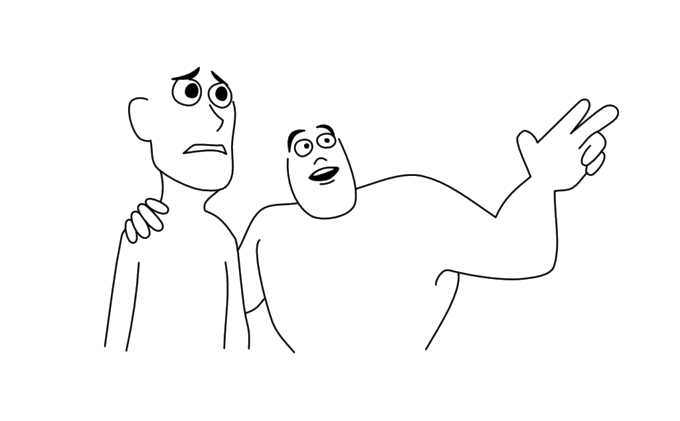
\includegraphics[width=0.5\textwidth]{../ressources/x-x-everywhere.png}
%     \vspace{-40pt}
%     \caption*{\tiny{Scalability everywhere.}}
%   \end{center}
%   \vspace{-40pt}
% \end{wrapfigure}

% I studied scalability in the domain of computer sciences.
% Scalability of the performance of an application over resources, as is often suggested when refering to scalability.
% But as well as scalability of the development project of such application.
% It now seems to me as if scalability is a crucial component of interacting and evolving in the world.
% From space exploration, to economical market ...
% \comment{What I take for scalability, might be overlapping with marginal increase, or incremental development}


This work is the fruit of a collaboration between the Worldline and the Inria DICE (Data on the Internet at the Core of the Economy) team from the CITI (Centre d’Innovation en Télécommunications et Intégration
de services) at INSA de Lyon.
For Worldline, this work fall within a larger work named Liquid IT, on the future of the cloud infrastructure and development.
As defined by Worldline, Liquid IT roughly aims at decreasing the time to market of a web service, allow the development team to focus on service specifications rather than technical twists and ease service maintenance.
The purpose of my work, was to separate development from performance scalability, to allow a continus development from prototyping phase, until runtime on thousands of clusters.
On the other hand, the DICE team focus on the consequences of technology on economical and social changes at the digital age.
This work falls as well within this scope as the development of web services is driven by economical factors.

\section{Web development}

The growth of web platforms is partially due to Internet's capacity to allow very quick releases of a minimal viable product (MVP).
In a matter of hours, it is possible to release a prototype and start gathering a user community around.
\textit{``Release early, release often''}, and \textit{``Fail fast''} are the punchlines of the web entrepreneurial community.
It is crucial for the prosperity of such project to quickly validate that the proposed solution meets the needs of its users.
Indeed, the lack of market need is the number one reason for startup failure.\ftnt{https://www.cbinsights.com/blog/startup-failure-post-mortem/}
That is why the development team quickly concretises an MVP and iterates on it using a feature-driven, monolithic approach.
Such as proposed by imperative languages like Java or Ruby.

\section{Performance requirements}

If the service successfully complies with users requirements, its community might grow with its popularity.
If it can quickly respond to this growth, it is scalable.
However, it is difficult to develop scalable applications with the feature-driven approach mentioned above.
Eventually this growth requires to discard the initial monolithic approach to adopt a more efficient processing model instead.
Many of the most efficient models distribute the system on a cluster of commodity machines.

Once split, the service parts are connected by an asynchronous messaging system.
Many tools have been developed to express and manage these service parts and their communications.
However, these tools impose specific interfaces and languages, different from the initial monolithic approach.
It requires the development team either to be trained or to hire experts, and to start over the initial code base.
This shift causes the development team to spend development resources in background without adding visible value for the users.
It is a risk for the evolution of the project as the number two and three reasons for startup failures are running out of cash, and missing the right competences.

\section{Problematic and proposal}

These shifts are a risk for the economaical evolution of a web application by disrupting the continuity in its developpement.
The main question I address in this thesis is how to avoid these shifts, so as to allow a continuous development?
That is to reconcile the reactivity required in the early stage of development and the performance increasingly required with the growth of popularity.
To answer this question, I propose in this thesis a solution based on an equivalence between two different programming paradigms.
On one hand, there is the imperative, functional, asynchronous programming model, embodied by Javascript.
On the other hand, there is the dataflow, distributed, programming model, embodied by the concept of fluxions introduced in chapter \ref{chapter5}.

This thesis contains two main contributions.
The first contribution is a compiler allowing to split a program into a pipeline of stages depending on a common memory store.
The second contribution, steming from the first one, is a second compiler, allowing to make the stages of this pipeline independent.
With these two contributions, it is possible to build a compiler that links an imperative representation with a flow-based representation.
The imperative representation carries the functional modularization of the application, while the flow-based representation carries its execution distribution.
A development team shall then use these two representations to continuesly iterate over the implementation of an application, while keeping both maintainability and performance.

% In this thesis, I study Javascript, as it seems to be increasingly used in web development, both client- and server-side, to start projects.
% Moreover, Javascript has the particularity to be implemented on top of an event-loop.
% % Javascript is the only language featuring such design and released at such scale, but it is by no mean limited to Javascript.
% This design is highly efficient and easy to develop with.
% But it remains limited to one core of a processor.
% Therefore, the problem of switching to a distributed approach remains.

% To give a first answer to this question, I limited this question to a problematic of compilation from Javascript to a distributed approach.
% More specifically, to a problem of memory analysis.
% In this thesis, I make two main contributions.
% The first contribution is a language and its execution engine to support the distributed approach.
% The second contribution is an equivalence between Javascript, or any similar language, and the language of the first contribution.

\section{Thesis organization}

This thesis is organized in four main chapters.
Chapter \ref{chapter2} introduces the context for this thesis and explains in greater details the objective I briefly described above.
It presents the challenge to build web applications scaling to world wide web, without jamming the organic evolution of its implementation.
It concludes drawing a first answer to this challenge.
Chapter \ref{chapter3} presents the works surrounding this thesis, and how they relate to it.
It defines into the notions outlined in the precedent chapter to help the reader understand better the context.
At the end of this chapter, I present clearly the problematic addressed in this thesis.
Chapter \ref{chapter4} presents the first contribution allowing to represent a program as a pipeline of stages.
We introduce Dues to encapsulate these stages, based on Javascript Promises.
Chapter \ref{chapter5} presents the second contribution allowing to make these stages independend.
We introduce Fluxion to encapsulate these stages.
Chapter \ref{chapter6} concludes this thesis, and draw the possible perspectives beyond this work.
